\documentclass[master=cws, masteroption=vs]{kulemt}

% Vul de titel van jouw masterproef hieronder in tussen { en }.
\setup{title={Gametheory and Cybersecurity: a study FlipIt and multiple resources},
%
% Vul hieronder namen in, steeds Voornaam Naam.
% Indien meerdere auteurs, assessoren, assistenten, scheidt hun namen
% met \and .
author={Sophie Marien},
promotor={Prof.\,dr.\,ir.\ Tom Holvoet},
assessor={Ir.\,W. Eetveel\and W. Eetrest},
assistant={Ir.\ Jonathan Merlevede, \ Ir. Kristof Coninx}}
% 
% De volgende \setup mag verwijderd worden als geen fiche gewenst is.
\setup{filingcard,
  translatedtitle={Beste masterproef ooit al geschreven},
  udc=621.3,
  shortabstract={Hier komt een heel bondig abstract van hooguit 500
    woorden. \LaTeX\ commando's mogen hier gebruikt worden. Blanco lijnen
    (of het commando \texttt{\string\pa r}) zijn wel niet toegelaten!
    \endgraf \lipsum[2]}}
% Verwijder de "%" op de volgende lijn als je de kaft wil afdrukken
%\setup{coverpageonly}
% Verwijder de "%" op de volgende lijn als je enkel de eerste pagina's wil
% afdrukken en de rest bv. via Word aanmaken.
%\setup{frontpagesonly}

% Kies de fonts voor de gewone tekst, bv. Latin Modern
\setup{font=lm}

% Hier kun je dan nog andere pakketten laden of eigen definities voorzien
\usepackage{graphicx}
\usepackage{amsmath}
\usepackage{listings}
\usepackage{color}
\usepackage{soul}
\usepackage{tikz}
\usepackage{parskip}
\usepackage{todonotes}
\usepackage{url}
\usepackage{natbib} 
\usepackage{pgf}
\usepackage{tikz}
\usetikzlibrary{arrows,automata}
%\usepackage[latin1]{inputenc}
\definecolor{dkgreen}{rgb}{0,0.6,0}
\definecolor{gray}{rgb}{0.5,0.5,0.5}
\definecolor{mauve}{rgb}{0.58,0,0.82}

\lstset{frame=tb,
  language=Java,
  aboveskip=3mm,
  belowskip=3mm,
  showstringspaces=false,
  columns=flexible,
  basicstyle={\small\ttfamily},
  numbers=none,
  numberstyle=\tiny\color{gray},
  keywordstyle=\color{blue},
  commentstyle=\color{green},
  stringstyle=\color{black},
  breaklines=true,
  breakatwhitespace=true
  tabsize=3
}

%\newcommand{\todo}[1]{{\huge \textcolor{green}{#1}}\\}
\newcommand{\com}[1]{\textcolor{red}{#1}\\}
\newcommand{\viscomment}[1]{\textcolor{red}{#1}}
\newcommand{\flip}[1] {\textcolor{black}{#1}}

% Tenslotte wordt hyperref gebruikt voor pdf bestanden.
% Dit mag verwijderd worden voor de af te drukken versie.
\usepackage[pdfusetitle,colorlinks,plainpages=false]{hyperref}

%%%%%%%
% Om wat tekst te genereren wordt hier het lipsum pakket gebruikt.
% Bij een echte masterproef heb je dit natuurlijk nooit nodig!
\IfFileExists{lipsum.sty}%
 {\usepackage{lipsum}\setlipsumdefault{11-13}}%
 {\newcommand{\lipsum}[1][11-13]{\par Hier komt wat tekst: lipsum ##1.\par}}
%%%%%%%

%\includeonly{chap-n}
\begin{document}

\begin{preface}
  I would like to thank everybody who kept me busy the last year,
  especially my promotor and my assistants. I would also like to thank the
  jury for reading the text. My sincere gratitude also goes to my wive and
  the rest of my family.
\end{preface}

\tableofcontents*
\listoftodos
\begin{abstract}
In this thesis I present a work of gametheory merged with cybersecurity. 
  The \texttt{abstract} environment contains a more extensive overview of
  the work. But it should be limited to one page.


\end{abstract}

\begin{abstract*}
  In dit \texttt{abstract} environment wordt een al dan niet uitgebreide
  Nederlandse samenvatting van het werk gegeven.
  Wanneer de tekst voor een Nederlandstalige master in het Engels wordt
  geschreven, wordt hier normaal een uitgebreide samenvatting verwacht,
  bijvoorbeeld een tiental bladzijden. 

  \lipsum[1]
\end{abstract*}

% Een lijst van figuren en tabellen is optioneel
%\listoffigures
%\listoftables
% Bij een beperkt aantal figuren en tabellen gebruik je liever het volgende:
\listoffiguresandtables
% De lijst van symbolen is eveneens optioneel.
% Deze lijst moet wel manueel aangemaakt worden, bv. als volgt:
\chapter{List of Abbreviations and Symbols}
\section*{Abbreviations}
\begin{flushleft}
  \renewcommand{\arraystretch}{1.1}
  \begin{tabularx}{\textwidth}{@{}p{12mm}X@{}}
    LoG   & Laplacian-of-Gaussian \\
    MSE   & Mean Square error \\
    PSNR  & Peak Signal-to-Noise ratio \\
  \end{tabularx}
\end{flushleft}
\section*{Symbols}
\begin{flushleft}
  \renewcommand{\arraystretch}{1.1}
  \begin{tabularx}{\textwidth}{@{}p{12mm}X@{}}
    42    & ``The Answer to the Ultimate Question of Life, the Universe,
            and Everything'' according to \cite{h2g2} \\
    $c$   & Speed of light \\
    $E$   & Energy \\
    $m$   & Mass \\
    $\pi$ & The number pi \\
  \end{tabularx}
\end{flushleft}

% Nu begint de eigenlijke tekst
\mainmatter

\chapter{Introduction}
\label{cha:intro}
The first contains a general introduction to the work. The goals are
defined and the modus operandi is explained.

\section{chap}

%%% Local Variables: 
%%% mode: latex
%%% TeX-master: "thesis"
%%% End: 

\chapter{Intoduction to GameTheory}
\label{Chapter1:Intro.Game.Theory}
%\documentclass[10pt]{article}
%\begin{document}

%%%%%%%%%%%%%%%%%%%%%%%%%%%%%%%%%%%%%%%%%%%%%%%%%%%%%%%%%%
%%%%%			Introduction Chapter 1				%%%%%%
%%%%%												%%%%%%
%%%%%												%%%%%%
%%%%%%%%%%%%%%%%%%%%%%%%%%%%%%%%%%%%%%%%%%%%%%%%%%%%%%%%%%

This chapter provides the reader with an introduction to the general context of the work presented in this paper.  Section 2.1 introduces the reader into the basic concepts of cyber security and the kind of cyber security threaths that are in the scope for this work. Section 2.2 then introduces the reader into the main principles of game theory. Subsequently, section 2.3 introduces the reader to the FlipIt game, the specific game that will be used to model cyber security attacks of periodic nature and including a delay.  Finally, section 2.4 gives an overview of the related work, and how the research presented in this thesis is positioned compared to existing results.

\section{What is cyber security?}

Before the digitalization of documents, information was kept on paper and the security of this information was ensured by administrative and physical means. For example, you needed a key to access documents stored in a room full of cabinets where the files were kept. In today's digital era more and more information is kept in a digital format, stored on a computer.  As digitalization progressed, the need for ensuring the security of digital information arose and automated tools where developed for protecting files stored on a computer.  The generic name to protect data stored on a computer controlled device such as computers and smartphones, as well as public and private computer networks, including the entire Internet is called computer security. 
Security is a general term that encompasses several dimensions. More specifically, computer security has tree key objectives that are fundamental to computer security:

~~\\
 \textit{Confidentiality}: This assures that the confidential of private data is not disclosed or made available to users that do not have the authorization. \\
 \textit{Integrity:} This assures that data can not be altered by an unauthorized individual.\\
 \textit{Availability:} This assures that data is always accessible and that the service is not denied to authorized individuals.\\


 %The purpose of security is to give certainty that data will not be removed without authorization (Confidentiality) that the data is always accessible (Availability), and that data can not be read or altered by someone who does not have the authorization (Integrity). 
 These are the 3 key attributes of security, also known as the CIA triad. The tree concepts are fundamental security objectives for the securing of data, information and computing services. \\
Cyber security is the process of applying security tools to ensure confidentiality, integrity, and availability of data. It is an attempt to protect websites, servers, data, applications, operating systems and all assets that need protection in a computer system.  Some of these tools may include detection, identification or removal tools. A detection tool will determine if an infection has taken place and will trace the threat. An identification tool will try to identify the threat to be able to know how to remove it. The removal tool will once the threat has been identified, remove the threat from the system so that it cannot spread any further. 

%Cybersecurity attempts to ensure the protection of assets, which includes data, desktops, servers, buildings, and most importantly, humans. The goal of cyber security is to protect data both in transit and at rest. Countermeasures can be put in place in order to increase the security of data. Some of these measures include, but are not limited to, access control, awareness training, audit and accountability, risk assessment, penetration testing, vulnerability management, and security assessment and authorization.'' \todo{tekst overgenomen van wikipedia} \\

\subsubsection{Threats to computer systems}


In order to keep a system secure and to be able to apply security tools, it is important to mitigate the possible threats. The possible threats can take many forms, the most common being spam, malware, spoofing, phishing and  DDoS attacks.  In the context of cyber security, the terms ' threat and attack' are often used interchangeably, referring to more or less the same thing. They however have a slightly different meaning. A threat refers to anything that can breach the security and that can cause a possible harm. It is a possible danger that can exploit a vulnerability. An attack is an assault on computer security that comes from a threat. It is an intelligent act that tries deliberately to breach security through vulnerabilities.  \\

The most noteworthy group and biggest group of threats to computer systems is malware. 
This is a piece of malicious software that is designed to penetrate unprotected systems or computers, with the intent to get sensitive information, destroy data, or compromise the confidentiality, integrity or availability of the data or applications of the victim. A security report of 2014 \cite{SurveyKaspersky} reveals that 61\% of the attacks on companies are caused by malware. For this reason this section will examine the categories of malware threats. Different types of malware exist such as virusses, worms, flooders, rootkits, bots, spyware, adware and many more. This broad range of different types can be classified into two main categories, the first one based on the propagation method that is used and the second one for the payload or the variety of actions that the malware performs. Propagation methods include virusses, worms and trojans. Payload includes flooders, rootkits, bots, spyware and adware. In this paper we focus on the category of propagation methods and not on the actions that the malware performs. We give a brief explanation of the three main propagation methods of malware. \todo{opsplitsing uit het boek van network security genomen}


\begin{description}
\item \textit{Virus}: This is a malicious piece of code that replicates itself and tries to spread in order  to infect other systems or files. A typical virus will attach itself to a program, or an executable content on a computer. The ''I love you'' virus is an example of a virus where the virus attached itself as an executable to a mail. To propagate it used the mail systems. If someone opens an email with the "I love you"  in the annex, the virus will spread itself by sending a mail to everyone in the victim's contact list. So the virus can multiply rapidly and eventually a business network might shut down by the heavy traffic. In this example, there is a need for human interaction to spread the virus. If no one opens the mail the virus can not spread itself and infect other systems.

\item \textit{Worm:} A worm is a virus that can spread without human interaction. A worm is a computer program that replicates itself in order to spread to other hosts on a network. Copies of the worm can be forwarded via a computer network without an intermediary. The worm will use vulnerabilities of the system to infect other computers.
The Stuxnetworm is a very prominent example of a worm. Initially this worm was spread via infected USB sticks and from there it could spread itself without any further human intervention through the Internet to other hosts on the network. The purpose of the Stuxnetworm was to harm the centrifuges in nuclear reactors and many reactors have been infected.  

\item \textit{Trojan:} This is a malicious program that disguises itself as something normal and useful, so that users won't be suspicious of installing it, but it has a malicious function hidden inside that can avoid security measures and cause harm.  A notable trojan horse is Koobface, that targeted users of facebook, skype, yahoo, gmail and AOL mail. To spread itself the worm sended a mail or friend request with a message that directed the recipients to another third party website. This site tried to put the reciepient into downloading an update of Adobe Flash Player. Once downloaded and executed, Koobface could infect the host. 

\end{description}

A company can take different measures to defend itself against malware. The threats caused by malware can be divided into three main categories: known threats (70\%), unknown threats (29\%) and advanced threats (1\%) as proposed by Kasperksy \cite{APTKaspersky}. 

The known threats are the easiest to defend oneself against. Standard malware protection tools like firewalls and virus scanners can keep these kind of malware out of the system. Installing protection against unkown is also relatively easy, but this will need tools that go beyond the standard methods like dynamic whitelisting. The remaining 1\% are the advanced threats, also known as APT.

\subsubsection{Advanced threats to computer systems}
%\item Backdoors: Also know as trapdoor, is a whole in the system or program that allows access 
%\item Rootkit: A rootkit is designed to be stealthy and hide a set of programs installed on a system from methods of detection.  The programs have administrator or root privileges to that system, which makes it possible to access the functions and services of the operating system, change files, take control over the monitor processes and send and receive network traffic.  A rootkit can make changes to the system to keep itself concealed from detection.

 An APT is a persistent targeted attack that tries to penetrate a network to cause harm while staying unseen for a long period of time. The motive of an APT is mostly cyber espionage, stealing sensitive data, sabotage or some other kind of ideological attacks. Advanced Persistent Threat are called  'Advanced' for the fact that these attacks are well funded and that (usually) the attacker itself needs a great expertise to successfully penetrate a network. Not all APTs are technical advanced though. The attacker can also try to exploit existing vulnerabilities simply based in the hope that his target has not yet secured himself against these vulnerabilities. 'Persistent' refers to the fact that the attacker keeps on trying to attack his target. The attack can be over various years and different steps can be taken. The 'threats' stands for the fact that an intelligent act tries deliberately to breach security through vulnerabilities which may severely damage the target organisation. 
An APT can be a mix of different types of malware and will use different kinds of propagation methods. \\
%
%Some examples of the biggest most rare APTs are listed to get an understanding of what APTs are capable of and how long they can stay unseen. [\todo{site kaspersky apt}] 
%
%\subsubsection{Equation}
%Equation is a complex cyberattack platform where the first known sample is from 2002, but it was only discovered 12 years later in 2014. This APT propagates through usb drives, cd or physical media. It will search for exploits and will self-replicate itself to spread the infection. The purpose of this virus is to steal data and cyberespionage. 
%
%\subsubsection{Regin}
%
%\subsubsection{Flame}
%Way of propagation through USB drives, LAN spreading. purpose cyber espionage.
%
%\subsubsection{Black energy}
% purpose cyber espionage and DDoS, data wiping. prop usb lan

 
According to a security survey of Kaspersky \cite{SurveyKaspersky}  the damage of one successful target attack against a large company can exceed over 2.54 million dollar. A company needs a defence mechanism to defend itself against APTs. As previously said, detection and identification tools will not work against APTs. The removal tool will only work if the threat has been identified. To mitigate these kind of attacks there is a need for another security countermeasures. Here is where the researchers of RSA fall in. They have investigated through game theory how to model targeted attacks and what the best defend strategy is according to the information that is available. 




\section{A brief introduction in Game Theory}
\label{Cha1:briefintro}
Gametheory is a mathematical study to analyse interactions between independent and self-interested agents. To get an understanding of the most important concepts of game theory, a short introduction based on the work of 
\cite{leyton2008essentials} and \cite{Coursera} is given in this section. For a more detailed and full introduction to game theory, the reader is referred to 
\cite{leyton2008essentials}.  \\
%In section \ref{cha1:FlipItGame} an overview of the FlipIt game is given with the definitions and concepts that will be used throughout the paper. 
%The last section \ref{ch1:extendedWork} will cover the extensions and additions already made on FlipIt. \\
%------------------------------------------------%
%            Intro Game Theory 					 %
%------------------------------------------------%





%begin over dat gametheorie handig is in de economie

Game theory studies the interaction between independent and self-interested agents. It is a mathematical way of modelling the interactions between two or more agents where the outcomes depend on what everybody does and how it should be structured to lead to good outcomes. It has therefore important applications in many area's such as economics, politics, biology, computer science, philosophy and a variety of other disciplines.  \\
%Every agent has different levels of happiness for the different outcomes.
%self interested meaning

One of the assumptions underlying game theory is that the players of the game, the agents, are independent and self-interested. This does not necessarily mean that they want to harm other agents or that they only care about themselves. 
%utility function meaning 
Instead it means that each agent has preferences about the states of the world he likes. These preferences are mapped to natural numbers and are called the utility function. The numbers are interpreted as a mathematical measure that tells how much an agent likes or dislikes the states of the world. \\
%Cooperative and non cooperative games
In a Decision Game Theoretic Approach an agent will try to act in such a way to maximise his expected or average utility function. It becomes more complicated when two or more agents want to maximise their utility and when actions of the agents can affect each other's utilities. This kind of games are referred to as non-cooperative game theory, where the basic modelling unit is the group of agents. The individualistic approach, where the basic modelling is only one agent, is referred as cooperative game theory. 

%There are two standard representations for games. The first one is the Normal Form. The second one is the Extensive Form.
 

%Nash equilibrium

%John Nash speelde ook een grote rol in de geschiedenis van de speltheorie. Hij is een van de wiskundigen geweest die speltheorie geformaliseerd heeft. Het Nash evenwicht werd naar hem vernoemd. Een Nash evenwicht wordt gezien als een evenwicht tussen beide spelers zodat ze allebei de beste tactiek kiezen en niet meer veranderen als de andere van tactiek veranderen. John Nash breide de theorie over het Nash evenwicht in een paper nog uit met gemengde strategieën. In 1994 kreeg John Nash samen met twee andere wiskundigen gespecialiseerd op het vlak van speltheorie de Nobelprijs voor de economie op basis van hun prestaties in de niet-coöperatieve speltheorie. . Over John Nash is een prachtige film 
\subsubsection{Best response and Nash Equilibrium}
One of the solution concepts in Game Theory for non-cooperative games is a Nash Equilibrium that will be used in this paper. A Nash Equilibrium is a subset of outcomes that can be interesting to analyse a game. To define this concept we first introduce the concept of best response. The best response for a player is the action of a player that maximizes it's pay-off for any given action of the other player. We define $Opt_{i}$ as the best response function for player \textit{i}. The best response for player \textit{1} is given by : $a_{1} = Opt_{1}(a_{2})$. A 
For a Nash Equilibrium each player has a consist list of actions and each player's action maximizes his or her pay-off given the actions of the other players. Nobody has the incentive to change his or her action if an equilibrium profile is played. We have a Nash Equilibrium for the pair $(a_{1}^{*},a_{2}^{*})$ where $a_{1}^{*} = Opt_{1}(a_{2}^{*})$ and $a_{2}^{*} = Opt_{2}(a_{1}^{*})$\\

\todo{optimal function same as best response ?}

%In game theory, the Nash equilibrium is a solution concept of a non-cooperative game involving two or more players, in which each player is assumed to know the equilibrium strategies of the other players, and no player has anything to gain by changing only their own strategy.[1] If each player has chosen a strategy and no player can benefit by changing strategies while the other players keep theirs unchanged, then the current set of strategy choices and the corresponding payoffs constitutes a Nash equilibrium. The reality of the Nash equilibrium of a game can be tested using experimental economics method.

%In de speltheorie, een deelgebied van de wiskunde, is een Nash-evenwicht een oplossingsconcept voor een niet-coooperatief spel, waar twee of meer spelers aan meedoen. In een Nash-evenwicht wordt elke speler geacht de evenwichtsstrategieeen van de andere spelers te kennen en heeft geen van de spelers er voordeel bij om zijn of haar strategie eenzijdig te wijzigen. Als elke speler een strategie heeft gekozen en geen enkele speler kan profiteren door zijn strategie te veranderen, terwijl de andere spelers dat ook niet doen, dan vormt de huidige verzameling van strategiekeuzes plus de bijbehorende uitbetalingen een Nash-evenwicht. 

%Een Nash-evenwicht gaat uit van een spel, waarin iedere speler een strategie heeft. Die strategie geeft precies aan wat een speler in de verschillende fases van een spel doet. Een strategie kan zowel een pure strategie als een gemengde strategie zijn. De verzameling van strategieeen van alle spelers die meedoen aan een bepaald spel noemt men een strategieprofiel. In de speltheorie is een Nash-evenwicht een strategieprofiel waarbij het voor geen enkele speler voordelig is daarvan af te wijken, als de andere spelers dat ook niet doen.

%Het Nash-evenwichtsconcept is een begrip dat vooral toepassing vindt in de economie.

\subsubsection{List of terms}
In the following list a couple of terms that will be used throughout the paper.
\begin{description}
\item \textit{Players}: Players are referred as the ones who are the decision makers. It can be a person, a company or an animal.  (they will act rational )
\item \textit{Actions}: Every player has actions that he or she can do. 
\item \textit{Strategies}: A strategy is the combination of different actions. A pure strategy is only one action.
\item \textit{Utility}: The utility function or also known as the pay-of is the mapping of the level of happiness of an agent about the state of the world to natural numbers.

\end{description}

A game in game theory consists of multiple agents and every agent has a set of actions that he can play.
\section{The FlipIt game}
\label{cha1:FlipItGame}
FlipIt is a game introduced by van Dijk et al. To understand how to model a FlipIt game with virus propagation it is important to get familiar with the concepts of the normal FlipIt game and its notations.  Therefore, we first explain the framework of FlipIt and introduce the most important formulas that will be used throughout the paper. \\

FlipIt is a two-players game with a shared single resource that the players want to control as long as possible. The shared resource can be a password, a network or a secret key depending on the setting being modelled. In the remainder of the paper we name the two players the attacker, denoted by the subscript \textit{A} and the defender, denoted by subscript \textit{D}. 

The game begins at $t=0$ and continues indefinitely ($t \rightarrow \infty $). The time in the game is assumed as being continuous. To get control over the resource, the players $i$, with $i \in \{A,D\}$, can flip the resource at any given time. 
%A flip will be regarded as a move from a player \textit{i}. 
Each move implies a certain cost $k_{i}$ and can vary for each player. Both players try to minimize their cost. Adding a cost prevents players to move too frequently. \\

The unique feature of FlipIt is that every move happens in a stealthy way, meaning that the player has no clue that the other player (his adversary) has flipped the resource. For instance, the defender does not find out if the resource has been compromised by the attacker until he flips the resource himself. The goal of the player is to maximize the time that he or she has control over the resource while minimizing the total cost of the moves. A move can also result in a "wasted move", called a flop. It may happen that the resource was already under control by the player. If the player moves when he or she has already control over the resource, he or she would have wasted a move since it does not result in a change of ownership, so the cost is wasted. \\


\begin{figure}[hbtp]
\centering
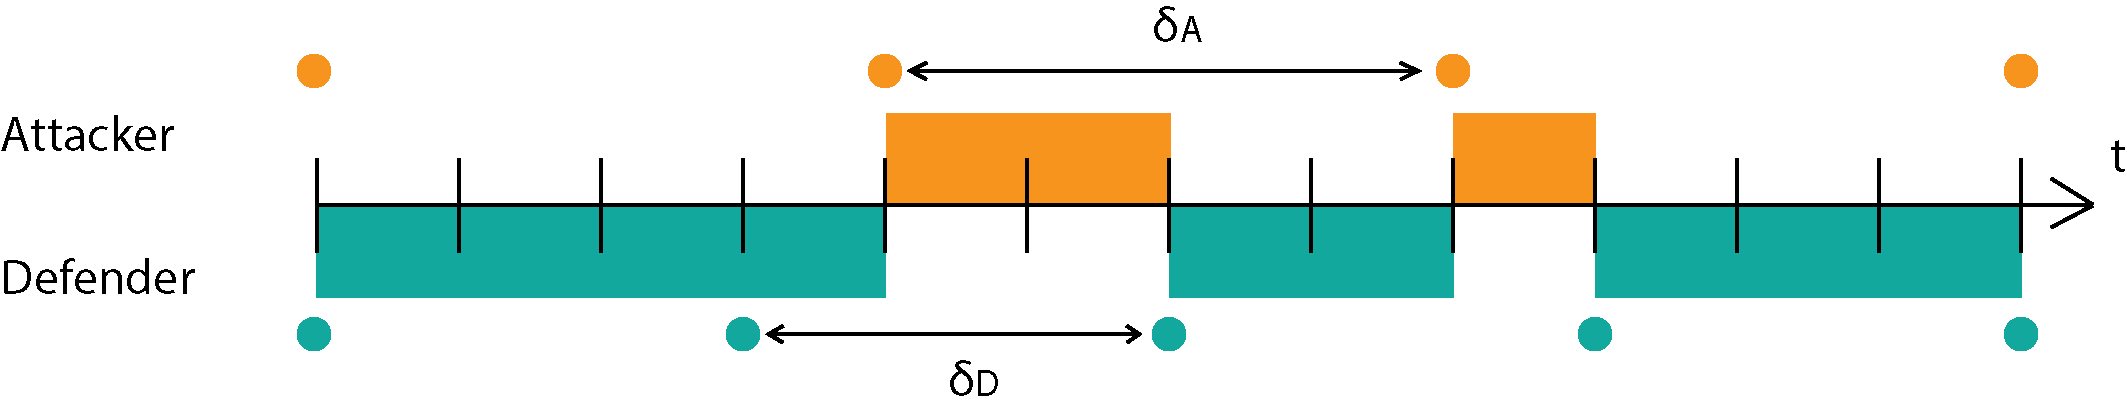
\includegraphics[scale=0.7]{../../doc/template/Images/FLipi.png}
\caption{A representation of a FlipIt game where both players are playing periodically. Every move or flip is indicated by a blue or orange circle. The attacker is represented in orange and plays with a period of $\delta_{A}=4$. The defender is represented in blue and plays with a period of $\delta_{D}=3$. The blue and orange rectangles represent the amount of time the respective player is in control of the resource.}
\label{fig:FLipItDefault}
\end{figure}



We denote the state of the resource as a time-dependent variable $C=C_{i}(t)$. 
$C_{D}(t)$ is 1 if the game is under control by the defender and 0 if the game is under control by the attacker. Reversely, $C_{A}(t)$ is 1 if the game is under control by the attacker and 0 if under control by the defender. So, $C_{A}(t)= 1 - C_{D}(t)$.
The game starts with the defender being in control: $C_{D}(0)= 1$. \\


The players receive a benefit equal to the time units they were in possession of the resource minus the cost of making their moves. The cost of a player \textit{i} is denoted by $k_{i}$. 
The total gain of player \textit{i} is equal to the total amount of time that a player \textit{i} has owned the resource from the beginning of the game up to time \textit{t}. It is expressed as follows:
\begin{equation}\label{first}
G_{i}(t) = \int_0^t \! C_{i}(x) dx.
\end{equation}
If we add up the gain of the defender and the gain of the attacker it should sum up to \textit{t}:
\begin{equation}\label{first}
G_{D}(t) + G_{A}(t) = t
\end{equation}
The average gain rate of player \textit{i} is defined as:
\begin{equation}\label{first}
\gamma_{i}(t) = G_{i}(t)/t.
\end{equation}
And thus for all $t > 0$ :
\begin{equation}\label{first}
\gamma_{D}(t) + \gamma_{A}(t) = 1
\end{equation}
Let $\beta_{i}(t)$ denote player's \textit{i} average benefit upto time \textit{t}:
\begin{equation}\label{first}
\beta_{i}(t) = \gamma_{i}(t) - k_{i}\alpha_{i}.
\end{equation}
This is equal to the fraction of time the resource has been owned by player \textit{i}, minus the cost of making the moves. ~$ \alpha_{i}$ defines the average move rate by player \textit{i} up to time \textit{t}.
In a given game, the asymptotic benefit rate (or simply benefit) will be defined as the lim inf of the average benefit because time\textit{ t} will increase to infinity and the average benefit may not have limiting values.
\begin{equation}
\beta_{i}(t)  = \lim_{t \to \infty} inf \beta_{i}(t) 
\end{equation}
\\


\subsubsection{strategies}
Because the players move in a stealthy way, there are different types of feedback that a player can get while moving. These types of feedback can be divided into two groups of strategies. The non-adaptive strategies and the adaptive strategies. These are described in table \ref{table:Strategies}. \\

If there is no feedback for either player, we have a non-adaptive strategy. Because a player does not receive any feedback during the game he will play in the same manner against every opponent. The strategy is called non-adaptive because the playing strategy is not dependent on the opponents movements. An interesting subclass of the non-adaptive strategies is the one where the time intervals between two consecutive moves are generated by a renewal process. An example of such renewal strategy is the periodic strategy where the time between two consecutive moves of the players are a fixed interval. An exponential strategy is a renewal strategy in which the interval between two consecutive moves is exponentially distributed. \\
In case there is feedback, a player can adapt his strategy to the information received about the opponent's moves. Depending on the amount of information received, two subclasses of adaptive strategies can be identified. The Last Move (LM) strategies represent the class where whenever a player flips he will find out the exact time that the opponent played the last time. In the second class, called Full History (FH), whenever a player flips he will find out the whole history of the opponent's move. \\
In this paper we restrict ourselves to periodic strategies. This choice is motivated by the fact that in a security game a player (defender or attacker) rarely has information about the moves (last move or full history) of his opponent.  \\


 \begin{table}
 \centering
 \begin{tabular}{ l | c  }
  \textbf{Categories} & \textbf{Classes of Strategies} \\
  \hline Non-adaptive (NA) & Renewal \\
  & - Periodic \\
  & ~~~ - Exponential \\
  & General non-adaptive \\
  \hline Adaptive (AD) & Last move (LM) \\
  & Full History (FH) \\  
\end{tabular}
 \caption{Hierarchy of Classes of strategies in FlipIt}
 \label{table:Strategies}
 \end{table}

\subsubsection{Results of the FlipIt game}
The study of the different strategies by means of FlipIt framework allows to derive a number of interesting results:  
\begin{itemize}
\item periodic games dominate the other renewal strategies, meaning that it is always advantageous to play periodically against an opponent with a renewal strategy;
\item periodic games are disadvantageous against players following a Last Move adaptive strategy;
\item if the defender plays with a periodic rate that is fast enough he'll force the attacker to drop out;
\item any amount of feedback about the opponent received during the game, benefits to a player.
\end{itemize}
 
 
\section{Extensions on FlipIt}
\label{ch1:extendedWork}

Various possible ways to extend FlipIt have already been proposed. 
Laszka et al. made a lot of additions and extensions to the original game of FlipIt. For instance Laszka et al. extended the basic FlipIt game to multiple resources. The rationale is that for compromising a system in real life, more than just one resource needs to be taken over. An example is that gaining access to deeper layers of a system may require breaking several passwords. The model is called FlipThem \cite{FlipThem}. Laszka et al. also use two ways to flip the multiple resources: the AND and the OR control model. In the AND model the attacker only controls the system if he controls all the resources of the system, whereas in the OR model the attacker only needs to compromise one resource to be in control of the entire system. \\

Another addition of Laszka et al. to the game of FlipIt \cite{MitigationCovert} 
is extending the game to also consider non-targeted attacks by non-strategic players. In this game the defender tries to maintain control over the resource that is subjected to both targeted and non-targeted attacks. Non-targeted attacks can include phishing, while targeted attacks may include threats delivered through zero day attack vulnerabilities. \\
One of the last important additions from Laszka et al. \cite{MitigationNonTargeted} is to consider a game with targeted and non-targeted attacks where the moves made by the attacker do not succeed immediately. This is similar to this paper but it has still some major differences. First the moves by the attacker are still covert but the moves made by the defender are known to the attacker. This means that the attacker knows when the defender plays and can change its strategy depending on the moves of the defender. Our motivation for a defender with stealthy moves is that there is not always an intelligent individual that is behind an APT. Some APTs don't know if the computer is already been recovered. There purpose is to spread. Not to check if they have already infected. \todo{beter verwoorden}. The second difference is that even though both the targeted and non-targeted attacks do not succeed immediately, the delay is determined differently. For the targeted attack the time till it succeeds is given by an exponential distributed random variable with a known rate. The non-targeted attacks are modelled as a single attacker and the time till it succeeds is given by a Poisson process. In our paper the delay is given by one parameter, that can be the result of any virus propagation model. The third and last difference is that the paper of Laska has multiple attackers and they try to find the best strategy of the defender against both targeted and non-targeted attacks. The conclusion of this paper is that the optimal strategy for the defender is moving periodically. \\ 

FlipIt has also been applied to several cases in system security. Reseachers explored different applications of FlipIt for real-world problems, like password reset policies, VM refresh, cloud auditing and key rotation \cite{ApplyingFlipit}. \\
Other authors used the FlipIt game to apply it on a specific scenario. To be able to use the FlipIt game, modifications where required for the FlipIt model.
One of the scenarios by Pham \cite{compromised} was to find out whether a resource was compromised or not by the attacker. This could be verified by the defender, who has an extra move "test" beside the flip move. The basic idea is to test with an extra action if the resource has been compromised or not. This move involves also an extra cost.\\
A three-player game has also been investigated where the flipit framework of two players is extended by another player. This player represents an insider that trades value information with the attacker \cite{fengstealthy}.\\


Finally researchers also have investigated the behaviour of humans playing FlipIt. A. Nochenson and Grossklags \cite{nochenson2013behavioral}  investigate how people really act when given temporal decisions. They found out that the results improves over time but that they are dependent on gender, age, and other individual difference variables. The result also shows that the participants perform generally better when they have more information about the strategy of the opponent which is a computerized player. Reitter et al. \cite{reitter2013risk} extended the work of A. Nochenson and Grossklags to include various visual presentation modalities for the available feedback during the investigation.\\




% --------------- example of a game -----------------%


%------------------------------------------------%
%            Intro about virusses				 %
%------------------------------------------------%


\chapter{The FlipIt game}
\label{cha:2}


\section{Extensions on FlipIt}

There a various possible ways to extend \flip{FlipIt}. For instance Laszka et al. extended the basic \flip{FlipIt} game to multiple resources. The incentive is that for compromising a system in a real case it needs more than just taking over one resource. An example is gaining access to a system and breaking the password. The model is called FlipThem \cite{FlipThem}. To ways of flipping the resources are used: the AND and the OR control model. In the AND model the attacker only controls the system if he controls all the resources of the system, whereas in the OR model the attacker only needs to compromise one resource to be in control of the entire system. The difference with FlipThem and this paper is that we introduce a Graph Model in the beginning.
Another extention on FlipIt is done by Pham [\todo{citatie needed voor Are We Compromised?}]. Beside the action Flip their is another action Test. The basic idea is to test with an extra action if the resource has been compromised or not. This action involves also an extra cost. This model is useful if somebody wants to know for example if his password has been compromised or wants to assess the periodic security of a system.  









In this section, we introduce the game \flip{FlipIt} \cite{FlipIt}. \flip{FlipIt} is a game introduced by .. .. and Rivest. First we explain the framework of FlipIt and after that the formulas and aannames that we will make for the game for during the whole paper.  

\section{The First Topic of this Chapter}
\flip{FlipIt} is a two-players game with a shared (single) resource that the players want to control as long as possible. The shared resource can be a password, a network or a secret key depending on the setting being modeled. In the rest of the paper we will call the players the Attacker and the Defender. To get the control over the resource, players can flip the resource at any given time. Each move will imply a certain cost. The unique feature of \flip{FlipIt} is that the move will happen in a stealthy way, meaning that the other player has no clue that the other player has flipped the resource. For instance, the defender will not find out if the resource has already been compromised by the attacker, but he can only potentially know it after he flips the resource himself. The goal of the player is to maximize the time that he or she has control over the resource while minimizing total cost of the moves. Players won't move to frequently. A move can also result in a "wasted move", in this paper called flop. It could be that the resource was for example already under control of the defender. If the defender moves when he or she has already the control over the resource, he or she would have a wasted move because it would not result in a change of ownership. 
 
Because the players move in a sthealty way, there are different types of feedback that a player can get while moving:
\begin{itemize}
\item Non-adaptive (NA): The player does not receive any feedback while flipping.
\item Last move (LM): The player finds out the exact time the opponent played the last time.
\item Full History (FH): The player finds out the complete history of the opponents move.
\end{itemize}
The game can be extended by the amount of information that a player receives. It can also be possible for a player to get information at the start of the game. Both interesting cases are:
\begin{itemize}
\item Rate-of-play (RP: The player finds out the exact rate of play of the opponent.
\item Knowledge-of-strategy (KS): The player finds out the complete information of the strategy that the opponent is playing.
\end{itemize}

In our assumption will the strategy of both players be non-adaptive. Non of the players has information of the strategy of the opponent. 


\subsection{An item}
A master thesis is never an isolated work. This means that your text must
contain references. On-line documents\cite{FlipThem} as well as
books\cite{DefendingAgainstUnknownEnemy} can be referenced. \cite{Craig2005}.

\section{Figures}
Figures are used to add illustrations to the text. The \fref{fig:logo} shows
the KU~Leuven logo as an illustration.
\begin{figure}
  \centering
  
\includegraphics{logokul}
  \caption{The KU~Leuven logo.}
  \label{fig:logo}
\end{figure}

\section{Tables}
Tables are used to present data neatly arranged. A table is normally
not a spreadsheet! Compare \tref{tab:wrong} en \tref{tab:ok}: which table do
you prefer?

\begin{table}
  \centering
  \begin{tabular}{||l|lr||} \hline
    gnats     & gram      & \$13.65 \\ \cline{2-3}
              & each      & .01 \\ \hline
    gnu       & stuffed   & 92.50 \\ \cline{1-1} \cline{3-3}
    emu       &           & 33.33 \\ \hline
    armadillo & frozen    & 8.99 \\ \hline
  \end{tabular}
  \caption{A table with the wrong layout.}
  \label{tab:wrong}
\end{table}

\begin{table}
  \centering
  \begin{tabular}{@{}llr@{}} \toprule
    \multicolumn{2}{c}{Item} \\ \cmidrule(r){1-2}
    Animal    & Description & Price (\$)\\ \midrule
    Gnat      & per gram    & 13.65 \\
              & each        & 0.01 \\
    Gnu       & stuffed     & 92.50 \\
    Emu       & stuffed     & 33.33 \\
    Armadillo & frozen      & 8.99 \\ \bottomrule
  \end{tabular}
  \caption{A table with the correct layout.}
  \label{tab:ok}
\end{table}

\section{Lorem Ipsum}
This section is added to check headers and footers. So this chapter must at
least contain three pages. To make sure that we get the required amount,
the \textsf{lipsum} package isn't used but the text is put directly in the
text.

\subsection{Lorem ipsum dolor sit amet, consectetur adipiscing elit}
Sed nec tortor id felis tristique sodales. Nulla nec massa eu dui fermentum
tincidunt. Integer ullamcorper ante eget eros posuere faucibus. Nam id
ligula ut augue pulvinar vulputate id at purus. Aenean condimentum tortor
eu mi placerat eget eleifend massa mollis. Nam est mi, sagittis quis
euismod eget, sagittis in nibh. Proin elit turpis, aliquam et imperdiet
sed, volutpat eu turpis.

Pellentesque vel enim tellus, vitae egestas turpis. Praesent malesuada elit
non nisi sollicitudin non blandit lacus tincidunt. Morbi blandit urna at
lectus ornare laoreet. Suspendisse turpis diam, lobortis dictum luctus
quis, commodo at lorem. Integer lacinia convallis ultricies. Sed quis augue
neque, eu malesuada arcu. Nullam vehicula, purus vitae sagittis pulvinar,
erat eros semper massa, eu egestas nibh erat quis magna. Cras pellentesque,
nisl eu dapibus volutpat, urna augue ornare quam, quis egestas lectus nulla
a lectus.

Vivamus dictum libero in massa cursus sed vulputate eros imperdiet. Donec
lacinia, libero ac lobortis egestas, nibh dui ornare arcu, luctus porttitor
velit massa sit amet quam. Maecenas scelerisque laoreet diam, vitae congue
quam adipiscing vitae. Aliquam cursus nisl a leo convallis eleifend
fermentum massa porta. Nunc libero quam, dapibus dapibus molestie sit amet,
faucibus vel nunc.

\subsection{Praesent auctor venenatis posuere}
Sed tellus augue, molestie in pulvinar lacinia, dapibus non ipsum. Fusce
vitae mi vitae enim ullamcorper hendrerit eu malesuada est. Proin iaculis
ante sed nibh tincidunt vel interdum libero posuere. Vivamus accumsan metus
quis felis congue suscipit dapibus enim mattis. Fusce mattis tortor eget
ipsum interdum sagittis auctor id metus.

Integer diam lacus, pharetra sit amet tempor et, tristique non lorem.
Aenean auctor, nisi eu interdum fermentum, lectus massa adipiscing elit,
sed facilisis orci odio a lectus. Proin mi nibh, tempus quis porta a,
viverra quis enim. In sollicitudin egestas libero, quis viverra velit
molestie eget. Nulla rhoncus, dolor a mollis vestibulum, lacus elit semper
nisi, nec sollicitudin sem urna eu magna. Nunc sed est urna, euismod congue
mi.

\subsection{Cras vulputate ultricies venenatis}
Vivamus eros urna, sodales accumsan semper vel, lobortis sit amet mauris.
Etiam condimentum eleifend lorem, ullamcorper ornare lectus aliquet vitae.
Praesent massa enim, interdum sit amet semper et, venenatis ut elit.
Quisque faucibus, quam ac lacinia imperdiet, nulla neque elementum purus,
tempus rutrum justo massa porta sapien. Vestibulum ante ipsum primis in
faucibus orci luctus et ultrices posuere cubilia Curae; Sed ultrices
interdum mi, et rhoncus sapien rutrum sed.

Duis elit orci, molestie quis sollicitudin sed, convallis non ante.
Maecenas tincidunt condimentum justo, et ultricies leo tristique vitae.
Vestibulum quis quam non lectus dapibus eleifend a vitae nibh. Nam nibh
justo, pharetra quis iaculis consequat, elementum quis justo. Etiam mollis
lacinia lacus, nec sollicitudin urna lobortis ac. Nulla facilisi.

Proin placerat risus eleifend erat ultricies placerat. Etiam rutrum magna
nec turpis euismod consectetur. Phasellus tortor odio, lacinia imperdiet
condimentum sed, faucibus commodo erat. Phasellus sed felis id ante
placerat ultrices. Aenean tempor justo in tortor volutpat eu auctor dolor
mollis. Aenean sit amet risus urna. Morbi viverra vehicula cursus.

\subsection{Donec nibh ante, consectetur et posuere id, tempus nec arcu}
Curabitur a tellus aliquet ipsum pellentesque scelerisque. Etiam congue,
risus et volutpat rutrum, est purus dapibus leo, non cursus metus felis
eget ligula. Vivamus facilisis tristique turpis, ut pretium lectus luctus
eleifend. Fusce magna sapien, ullamcorper vitae fringilla id, euismod quis
ante.

Phasellus volutpat, nunc et pharetra semper, sem justo adipiscing mauris,
id blandit magna quam et orci. Vestibulum a erat purus, ut molestie ante.
Vestibulum ante ipsum primis in faucibus orci luctus et ultrices posuere
cubilia Curae; Proin turpis diam, consequat ut ullamcorper ut, consequat eu
orci. Sed metus risus, fringilla nec interdum vel, interdum eu nunc.
Suspendisse vel sapien orci.

\subsection{Morbi et mauris tempus purus ornare vehicula}
Mauris sit amet diam quam, eget luctus purus. Sed faucibus, risus semper
eleifend iaculis, mi turpis bibendum nisl, quis cursus nibh nisl sit amet
ipsum. Vestibulum tempor urna vitae mi auctor malesuada eget non ligula.
Nullam convallis, diam vel ultrices auctor, eros eros egestas elit, sed
accumsan arcu tortor eget leo. Vestibulum orci purus, porttitor in pharetra
eget, tincidunt eget nisl. Nullam sit amet nulla dui, facilisis vestibulum
dui.

Donec faucibus facilisis mauris ac cursus. Duis rhoncus quam sed nisi
laoreet eu scelerisque massa tincidunt. Vivamus sit amet libero nec arcu
imperdiet tempor quis non libero. Sed consequat dignissim justo. Phasellus
ullamcorper, velit quis posuere vulputate, felis erat tincidunt mauris, at
vestibulum justo lectus et turpis. Maecenas lacinia convallis euismod.
Quisque egestas fermentum sapien eu dictum. Sed nec lacus in purus dictum
consequat quis vel nisl. Fusce non urna sem. Curabitur eu diam vitae elit
accumsan blandit. Nullam fermentum nunc et leo dictum laoreet. Donec semper
varius velit vel fringilla. Vivamus eu orci nunc.

\section{Conclusion}
The final section of the chapter gives an overview of the important results
of this chapter. This implies that the introductory chapter and the
concluding chapter don't need a conclusion.

\lipsum[66]

%%% Local Variables: 
%%% mode: latex
%%% TeX-master: "thesis"
%%% End: 

%\chapter{Intoduction to GameTheory}
%\label{cha:1}
\documentclass[10pt]{article}
\begin{document}



\section{Write down the settings of the game}

What is different from Flip-It.

%%% Local Variables: 
%%% mode: latex
%%% TeX-master: "thesis"
%%% End: 

\end{document}

% ... en zo verder tot
\chapter{The Final Chapter}
\label{cha:n}


\section{chap}

%%% Local Variables: 
%%% mode: latex
%%% TeX-master: "thesis"
%%% End: 

\chapter{Conclusion}
\label{cha:conclusion}
The final chapter contains the overall conclusion. It also contains
suggestions for future work and industrial applications.

\lipsum[1-7]

%%% Local Variables: 
%%% mode: latex
%%% TeX-master: "thesis"
%%% End: 


% Indien er bijlagen zijn:
\appendixpage*          % indien gewenst
\appendix
\chapter{The First Appendix}
\label{app:A}
Appendices hold useful data which is not essential to understand the work
done in the master thesis. An example is a (program) source.
An appendix can also have sections as well as figures and references.

\section{More Lorem}


%%% Local Variables: 
%%% mode: latex
%%% TeX-master: "thesis"
%%% End: 

% ... en zo verder tot
\chapter{The Last Appendix}
\label{app:n}
Appendices are numbered with letters, but the sections and subsections use
arabic numerals, as can be seen below.

\section{Lorem 20-24}


%%% Local Variables: 
%%% mode: latex
%%% TeX-master: "thesis"
%%% End: 


\backmatter
% Na de bijlagen plaatst men nog de bibliografie.
% Je kan de  standaard "abbrv" bibliografiestijl vervangen door een andere.
\bibliographystyle{abbrv}
\bibliography{references}

\end{document}

%%% Local Variables: 
%%% mode: latex
%%% TeX-master: t
%%% End: 

